\documentclass[letter, 11pt] {article}

\usepackage{tabularx}
\usepackage{graphicx}
\usepackage[french]{babel}
\usepackage[utf8]{inputenc}
\usepackage[french, vlined]{algorithm2e}
\usepackage{geometry}
\geometry{ hmargin=2.5cm, vmargin=2.3cm }

%%%%% Page titre %%%%


%%%% Résumé %%%%
%Pour la taille des interlignes
\renewcommand{\baselinestretch}{1.3}


\newlength{\larg}
\setlength{\larg}{15cm}

\title{
{\rule{\larg}{1mm}}\vspace{7mm}
\begin{tabular}{p{0cm} r}
& {\Huge {\bf Rapport d'activité}} \\
\end{tabular}\\
\vspace{2mm}
{\rule{\larg}{1mm}}
\vspace{2mm} \\~\\
\begin{tabular}{p{3cm} r}
& {\large \bf Projet transversal de conception objet - IG4} \\
& {\large \bf encadré par M. Sala} \\
& {\large 17 mars 2011}
\end{tabular}\\
\vspace{10cm}
}
\author{\begin{tabular}{p{5cm} l}
 Emmanuel Damiano & Quentin Dejean\\ 
 Raphael Pastou & Damien Vacher
\end{tabular}\\
\hline }
\date{}

\begin{document}

\maketitle
\thispagestyle{empty}

\setcounter{page}{1}

	\section*{Introduction}
	
	Dans le cadre de notre quatrième année à l'école d'ingénieur de Polytech' Montpellier, en informatique et gestion, il nous a été demandé de réaliser un projet transversal.

	Ce projet se basait sur la conception d'un logiciel pour la gestion des notes à Polytech' Montpellier. Autrement dit, pour l'ensemble des étudiants de l'école, il fallait pouvoir récupérer et saisir leurs notes sur une plateforme internet. Les moyennes de chaque matière sont ramenées par les professeurs aux secrétaires, qui doivent rentrer ces notes sur la plateforme dédiée.

	En plus de cette saisie, une gestion des responsables de chaque filière devait être implémentée, permettant aux utilisateurs de pouvoir consulter depuis leurs ordinateurs les notes de leurs étudiants.

	Un premier rapport d'activité a été établi et rendu pour le premier semestre. Celui-ci nous a permis de poser les bases de la conceptions : nous avons déterminé avec précision les besoins de l'utilisateur, par le biais d'un cahier des charges que nous avons nous-mêmes établi. A la suite de quoi nous avons réalisé la conception à l'aide de différents diagrammes UML. Tout d'abord, nous avons créé le diagramme des classes correspondant aux besoins du logiciel, puis les diagrammes de cas d'utilisation qui retranscrivent les futures besoins à réaliser.

	A la suite de ce premier rendu vient une nouvelle étape de la conception. Toutefois, celle-ci est plus proche de la programmation, plus technique.Cela nous permet de cerner et analyser les différentes phases de développement que nécessite le projet, et les diverses fonctionnalités utilisées.

	Voici donc le rapport présentant les différents diagrammes de la seconde étape du développement, accompagné du diagramme de classes et des diagrammes d'utilisation revus et corrigés.
	
	\newpage
	
	\tableofcontents
	
	\section{Le diagramme de classes}
	
	\begin{figure}[!h]
		\centering
			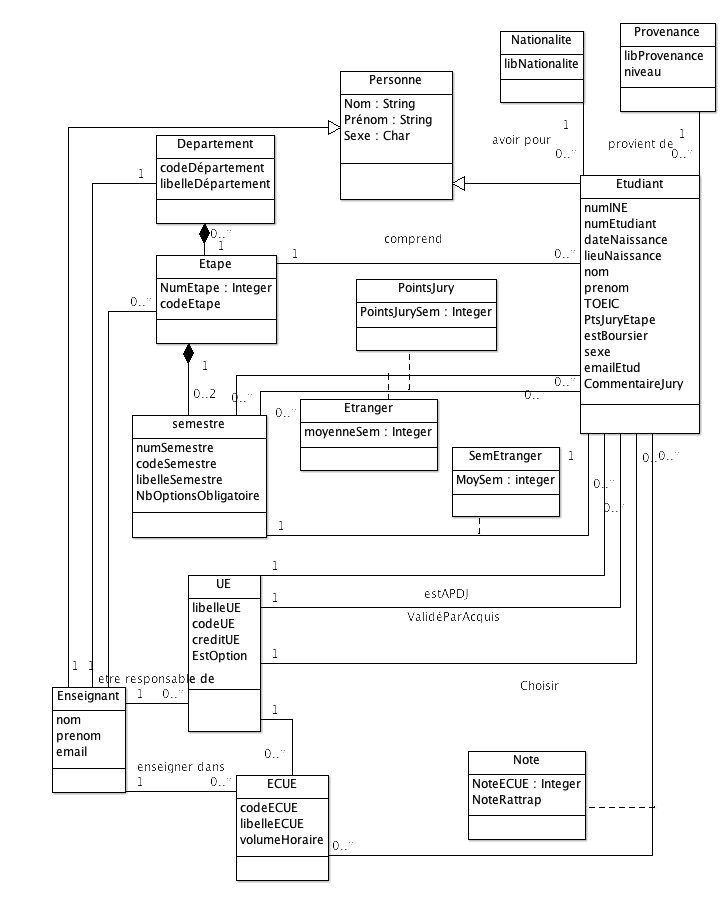
\includegraphics[scale = 0.7]{../Diagramme_de_classes/Diagramme_classe.png}
	\end{figure}
	
	\paragraph{ }Afin de mieux comprendre le diagramme des classes que nous avons établi, il est nécessaire de s'attarder sur une légère description des classes et surtout des relations entre elles. Nous allons donc expliquer nos choix en décrivant pas à pas les étapes de notre réflexion.

	\paragraph{ }Le projet s'appuie sur une gestion des notes des étudiants de Polytech'. Cette école est polytechnique, et propose donc divers départements correspondant à des cursus scolaires différents. Une classe « Diplôme » nous a donc parue essentielle pour la gestion du problème. Cette classe représentera les différents départements de l'école (IG, ERII, STIA,…), identifiables grâce à l'attribut « Libellé\_Diplôme » et la classe en elle-même sera identifiable par un attribut « Code\_Diplôme ». Bien entendu, le diplôme passé par les étudiants de chaque filiale ne s'obtient généralement pas en une année. Il fallait donc ici gérer l'ensemble des étapes d'un département (IG3, IG4, IG5, ERII3, ERII4,…), d'où la création d'une classe « Étape » , comprenant un « Libelle\_Étape » répertoriant les diverses étapes et un attribut « Code\_Étape » afin de différencier les différentes années. Bien entendu, une étape n'appartient qu'à un seul diplôme, et ce dernier contient plusieurs étapes (généralement trois) ce qui justifie les cardinalités proposées. De plus, si un diplôme venait à disparaître, suppression de ERII par exemple, il est compréhensible que les différentes étapes qui composaient ce diplôme (ERII3, ERII4 et ERII) viendraient à être supprimées également. C'est pourquoi nous avons utilisé ici une relation « Composition »  pour appuyer sur la dépendance entre les deux classes.

	\paragraph{ }Nous allons à présent détailler les différentes classes liées à une étape. En effet, une étape est composée d'un ou plusieurs semestre, généralement deux - sauf pour les FQSC. Mais ce nombre pourrait être augmenté : nous avons donc voulu créé entre ces classes une relations permettant de lier plus de deux semestres à une étape. De plus, une étape a un responsable, qui est nécessairement un professeur dirigeant une matière de l'étape, chargé lui-même du suivi des élèves. Laisser une étape sans responsable est impensable, c'est pourquoi nous avons décidé d'attribuer à la relation entre Étape et Enseignant une cardinalité signifiant qu'une Étape était dirigée par un et un seul enseignant (ce dernier pouvant diriger zéro ou plusieurs étapes).

	\paragraph{ }Comme nous venons de le voir, une étape regroupe plusieurs semestres. Un semestre dure généralement la moitié de l'année (sauf FQSC) et est identifié par un « Code\_Semestre » (premier ou deuxième semestre d'une étape) ainsi qu'un « Libelle\_Semestre » comportant les informations sur le semestre. Un semestre se compose de plusieurs UE, ces dernières pouvant appartenir à plusieurs semestres (dans le cas d'UE transversales par exemple). De plus, pour un semestre donné, un ensemble d'étudiants est évalué (à la fin de chaque semestre grâce à l'ensemble des notes obtenues pendant celui-ci). Cette évaluation est dans un premier temps la moyenne des notes d'UE d'un étudiant. Néanmoins, cet attribut étant calculable il n'est ici pas mentionné. Toutefois, un étudiant peut voir son parcours sur le semestre évalué par un jury, et ce  dernier pourra accorder des  « points jury » pour permettre la validation du semestre (ces points s'ajoutent à la moyenne générale). Il faut donc tenir compte de ces points. C’est pourquoi nous avons ajouté un attribut à la relation « Suit », permettant de répertorier les points jury des étudiant pour un semestre et de les inclure dans le calcul de sa moyenne. Pour finir, chaque étudiant suit un ou deux semestres par étape. Et étant donné que le logiciel doit gérer les élèves année par année, la cardinalité « 1..2 » est justifiée. En effet, il peut arriver qu’un élève ne suive pas réellement un semestre (remplacé par un stage par exemple dans le cas de 

	\paragraph{ }Nous allons à présent revenir sur la classe « enseignant ».  Comme nous l'avons expliqué, un enseignant peut diriger une ou plusieurs étapes. Mais il peut également être responsable d'une ou plusieurs UE (à condition d'être responsable d’une ECUE de l'UE) ou d’une ou plusieurs ECUE . Afin d'avoir certaines informations sur un enseignant, nous gardons dans la classe son nom, prénom, mais surtout son login et mot de passe lui permettant de se connecter au système (pour consulter les résultats de ses étudiants par exemple).
	\paragraph{ }	Dans l'organisation de l'école, la principale structure est celle des UE (Unité d'Enseignement). Une UE et un agglomérat de plusieurs matières (ECUE) proposant un cursus portant sur des connaissances proches et liées. Ces matières comportant un « code ECUE » composé en partie du « code UE », elles ne peuvent avoir une existence propre si l'UE à laquelle elles appartiennent est détruite. Ceci explique la composition qui les relie à une UE. Une UE est également soumise à un type d'obligation. En effet, lors de certaines étapes, certaines UE peuvent être optionnelles, ce qui explique la création d'une classe « Type\_UE » qui contiendra comme « libelle\_Obligation » « Obligatoire » ou « Optionnelle ». Comme nous l'avons vu précédemment, une UE peut appartenir à zéro ou plusieurs semestres. Nous avons détaillé ce processus précédemment et ne reviendrons donc pas dessus. Pour terminer, nous allons nous intéresser aux notes obtenues par un étudiant dans les UE, c'est-à-dire la moyenne de leurs notes dans chaque matière de l’UE.  Néanmoins, cet attribut est calculable et n'apparaîtra pas dans le diagramme. Il est toutefois nécessaire d’y faire apparaître l’  « Evaluation\_UE ». Cette dernière est certes calculable, en vérifiant si la moyenne est supérieure à dix, mais peut être modifiable par le jury. La moyenne est alors conservée mais on modifie la « Decision\_Jury » (qui peut être ACDJ, Acquis, AJ, … ». Un étudiant pouvant être inscrit et noté dans zéro ou plusieurs UE, et une UE regroupant toute une promotion (voire plusieurs), donc un ensemble d'étudiants, les cardinalités sont expliquées. La classe « UE » contient également un « libelle\_UE » afin de stocker le nom de l’UE (mathématiques, algorithmique, ...).

	\paragraph{ }	La deuxième structure importante est l'ECUE, ou matière. Une matière peut être enseignée par plusieurs professeurs mais dirigée par un seul (d’où la cardinalité sur « dirige\_ECUE ». De plus, une matière est soumise à un code (code UE + code) et pèse un certain poids dans la notation finale, poids calculé à partir des « crédits\_ECUE » qu'offre la validation de l'ECUE. Pour finir, nous répertorions aussi le « libelle\_ECUE » qui correspond au nom de la matière.

	\paragraph{ }	Bien entendu, le système doit gérer le suivi des notes d’un étudiant. Il est donc primordial d'avoir une classe « Etudiant ». Cette classe possède les informations essentielles d’un étudiant (nom, prénom, date de naissance et numéro INE, sexe, nationalité ainsi que formation antérieure), ainsi que le type de bourse qu’il possède, afin notamment de permettre les statistiques et la gestion des stages. Un étudiant est donc - comme vu précédemment - inscrit dans des UE. Mais il doit également participer à toutes les ECUE des UE dans lesquelles il est inscrit. Pour chaque ECUE, l’étudiant sera noté, et nous stockerons donc ses notes dans l'attribut de relation « Evaluation\_ECUE». Mais le système de Polytech’ possède une particularité : pour valider son diplôme, un élève doit obligatoirement obtenir une certification dans une langue étrangère (Anglais, espagnol, arable, …). C’est pourquoi nous avons rajouté une classe « Certificat », qui stockera l’ensemble des certifications possibles. Un étudiant peut passer des épreuves correspondant à un ou plusieurs certificats, et il obtiendra pour chaque épreuve une note. Nous ne garderons toutefois que la meilleure note obtenue pour chacune des certifications, d’où l’attribut de relation « Evaluation Certification ».
	
	\section{Les cas d'utilisation}
	
	Tout comme a été présenté le diagramme de classe, voici les diagrammes d'utilisation que nous avons réalisé.  
	
	\section{Les cas d'utilisation de la secrétaire}
	
	La principale personne ayant à utiliser le logiciel sera le secrétaire. C'est en effet cette personne qui devra, en plus de la consultation de données, effectuer des insertions/modifications de profil, ainsi que l'insertion des notes au sein de la base. Nous allons donc nous pencher plus particulièrement sur tout les cas d'utilisation que le secrétaire pourrait être amené à effectuer.

	\subsection{Les diagrammes de haut niveau}
	
	
	Le premier cas d'utilisation que nous avons recensé est le choix concernant le type d'action à effectuer. Dans la Figure 1 ci-dessous, nous pouvons donc observer que le secrétaire pourra consulter, modifier ou supprimer des informations concernant le système. Nous entendons par là, comme vous le verrez par la suite, insérer des notes ou des enseignant, modifier des notes, données ou structure, et consulter l'intégralité des informations du système.
	
		\begin{figure}[!h]
			\centering
				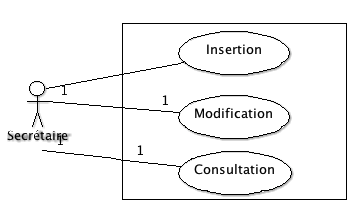
\includegraphics[scale = 0.7]{../UseCase/UseCaseHautNiveau/UseCase_HautNiveau_General.png}
			\caption{Diagrammes représentant les cas d'utilisation au plus haut niveau}
		\end{figure}
		
		
	\subsubsection{La consultation d'informations}
	
	Trois types d'action principales sont à noter, concernant la consultation d'informations. Comme montré dans la figure 3 ci-dessous, trois types de consultation sont attendues.
			
	\begin{figure}[!h]
		\centering
			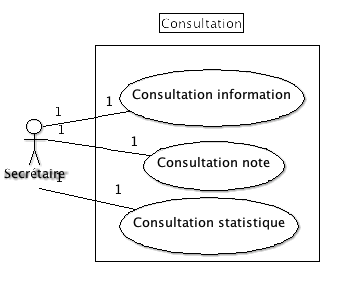
\includegraphics[scale = 0.7]{../UseCase/UseCaseHautNiveau/Consultation.png}
		\caption{Diagrammes représentant les cas d'utilisation au plus haut niveau}
	\end{figure}
	
	Premièrement, le secrétaire pourrait vouloir consulter certaines informations : profil d'un responsable ou d'un étudiant, ou bien certaines structures d'enseignement.
	
	Dans un deuxième temps, la secrétaire pourrait avoir à consulter les notes des étudiants. 
La consultation doit permettre également l'édition des relevés de notes, par promotion et par étudiant, par semestre, UE, ECUE ou encore par certificat, tout en sachant que la consultation par UE n'est possible que si l'ensemble des ECUE de l'UE ont une note.
	
	Pour terminer en ce qui concerne la consultation à haut niveau, une consultation des différentes statistiques des étudiants pourrait être nécessaire, selon les informations insérées dans la base sur ces derniers.
	
	\subsubsection{L'insertion d'informations}
	
	Comme décrit dans la figure 4 ci-dessous, il se peut que la secrétaire ait différentes insertions à effectuer.
	
	\begin{figure}[!h]
		\centering
			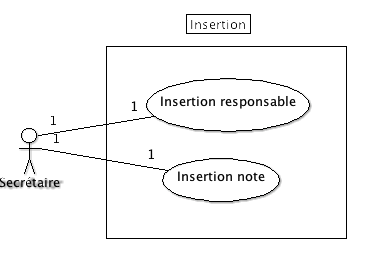
\includegraphics[scale = 0.5]{../UseCase/UseCaseHautNiveau/Insertion.png}
		\caption{Diagrammes représentant les cas d'utilisation au plus haut niveau}
	\end{figure}
	\newpage
En effet, seul la  secrétaire a un accès à l'insertion de profils ainsi qu'à l'insertion des
notes des étudiants. C'est pourquoi le système lui permet d'insérer de nouveaux enseignants
dans la base, enseignant qu'elle pourra relier à certaines structures afin d'indiquer
leurs responsabilités, nous verrons cela par la suite. De plus, elle dispose du droit d'insérer
les notes des étudiants, manuellement ou par feuille excel, dans la base.
	
	\subsubsection{La modification d'informations}
	
	Là aussi, différentes actions principales peuvent être nécessaires au secrétaire.
	
	\begin{figure}[!h]
		\centering
			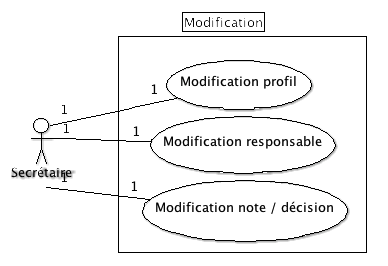
\includegraphics[scale = 0.7]{../UseCase/UseCaseHautNiveau/Modification.png}
		\caption{Diagrammes représentant les cas d'utilisation au plus haut niveau}
	\end{figure}
	
	Comme décrit dans la figure 5, le secrétaire pourrait avoir pour charge de modifier un profil enregistré au sein de la base. Par exemple, il pourrait avoir à mettre à jour des données concernant un responsable.
	
	De plus, il pourrait aussi être nécessaire de modifier la responsabilité d'un enseignant. Que ce soit pour sa première affectation, ou bien une modification d'un poste en plein milieu d'année, la secrétaire aura à sa disposition divers outils au sein du logiciel.
	
	Pour terminer, il se peut qu'un responsable ou bien encore qu'une décision du jury veuille modifier la note d'un étudiant, voire la décision prise concernant ce dernier. Il pourra donc modifier une note, ou bien la décision calculée par le logiciel.
	
	
	~\\
	
	Bien entendu, des utilisations plus poussées du logiciel pourrait être nécessaire pour la secrétaire. Aussi, la partie ci-dessous permet d'entrevoir certaines de ces possibilités.
	
	\subsection{Les diagrammes de niveau moyen}
	
		A un niveau plus bas que celui des uses cases précédemment décrit, les procédures sont plus détaillées, et de nouvelles entrent en jeu.
		
		\subsubsection{L'insertion d'informations}
		
			\paragraph{L'insertion de données pour un responsable}
~\	\paragraph{ }	Comme vous pouvez le voir dans la figure 6 ci-dessous, différentes données concernant les responsables peuvent être insérées. Tout d'abord, il peut simplement s'agir de l'insertion d'un nouvel enseignant au sein de la base. Auquel cas le secrétaire aura besoin du nom et du prénom de celui-ci.
		
		\begin{figure}[!h]
			\centering
				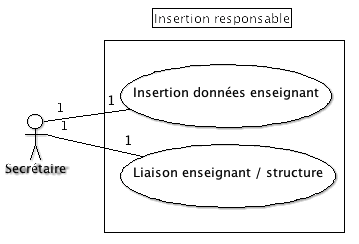
\includegraphics[scale = 0.7]{../UseCase/UseCaseMoyenNiveau/InsertionResponsable.png}
			\caption{Diagrammes représentant les cas d'utilisation à moyen niveau}
		\end{figure}
		
		Autrement, toujours à niveau moyen, lorsque l'enseignant est créé, le secrétaire aura besoin d'effectuer la liaison entre le le professeur et le poste de responsabilité qui doit lui être attribué. Toutefois, il ne faut pas oublier que pour obtenir un poste de responsable d'UE ou d'année, l'enseignant doit obligatoirement être responsable d'une matière.
		
		\newpage
			\paragraph{L'insertion d'une note}~\		\paragraph{ }Comme décrit plus haut, c'est le secrétaire qui insère toutes les notes des étudiants. Pour cela, il doit sélectionner soit une structure d'enseignement, plus communément appelée une matière. A partir de là, le secrétaire peut insérer la note d'un étudiant en particulieur ou pour une structure particulière.
		
			\begin{figure}[!h]
				\centering
					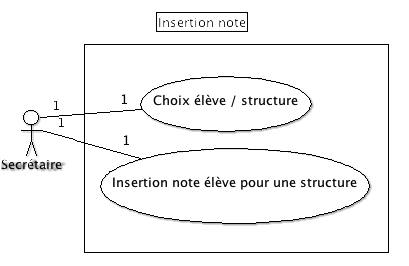
\includegraphics[scale = 0.6]{../UseCase/UseCaseMoyenNiveau/InsertionNote.png}
				\caption{Diagrammes représentant les cas d'utilisation à moyen niveau}
			\end{figure}
			
			Autrement, le secrétaire peut sélectionner directement l'étudiant et lui attribuer la note.
			
			
		\subsubsection{La modification d'informations}
		
			\paragraph{Modification d'un profil}~	\paragraph{ }La modification d'un profil concerne uniquement les enseignants. Bien que ceci devrait être un cas rare, il se peut toutefois que le secrétaire ait besoin de modifier les données dans le courant de l'année.
			
			\begin{figure}[!h]
				\centering
					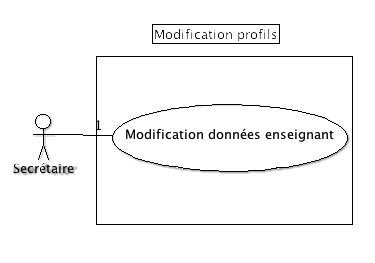
\includegraphics[scale = 0.5]{../UseCase/UseCaseMoyenNiveau/ModificationProfil.png}
				\caption{Diagrammes représentant les cas d'utilisation à moyen niveau}
			\end{figure}
			
			\newpage
			\paragraph{Modification d'un responsable}~\paragraph{ }Autre que la modification d'un profil, le secrétaire peut avoir à modifier directement le poste de responsabilité. Pour cela, comme décrit dans la figure ci-dessous, le secrétaire peut choisir une structure ou bien un responsable. 
			
			\begin{figure}[!h]
				\centering
					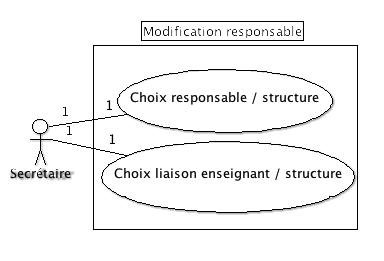
\includegraphics[scale = 0.5]{../UseCase/UseCaseMoyenNiveau/ModificationResponsable.png}
				\caption{Diagrammes représentant les cas d'utilisation à moyen niveau}
			\end{figure}
			
			Une fois que l'un ou l'autre a été sélectionné, il suffit de sélectionner respectivement le responsable, ou bien la structure associée.
			
			\paragraph{Modification d'une note ou d'une décision}~	\paragraph{ } La modification d'une note ou d'une décision d'un jury se déroule de la même manière que pour un responsable. Tout d'abord, on peut soit sélectionner une structure, soit choisir directement l'étudiant concerné. 
			
			\begin{figure}[!h]
				\centering
					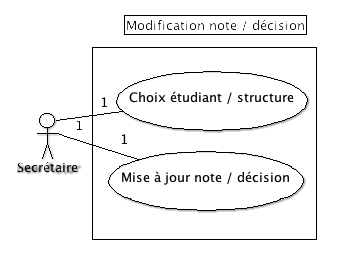
\includegraphics[scale = 0.5]{../UseCase/UseCaseMoyenNiveau/ModificationNoteDecision.png}
				\caption{Diagrammes représentant les cas d'utilisation à moyen niveau}
			\end{figure}
			
			Une fois l'étudiant sélectionné, on modifie alors la note, ou bien la décision du jury prise à son encontre.
	
\newpage
	\subsection{Les diagrammes de bas niveau}
	
		\subsubsection{Navigation}

			\paragraph{Consultation par navigation} Comme le montre la figure ci-dessous, pour consulter l'information désirée, le secrétaire devra spécifier sa cible c'est-à-dire un étudiant ou une structure. Il aura alors accès, en fonction de son choix, soit à la structure si un élève a été choisi en premier, soit à la liste des élèves si la structure dans le cas contraire.
Ce cas d'utilisation donnera lieu à un diagramme de séquence dans la suite du projet pour permettre un niveau de détail plus important.
		\begin{figure}[!h]\centering
				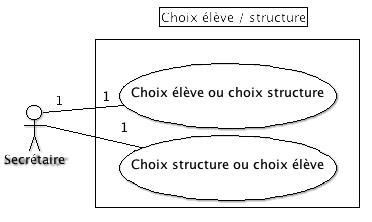
\includegraphics[scale = 0.5]{../UseCase/UseCaseBasNiveau/ChoixEleveStructure.png}
					\caption{Diagrammes représentant les cas d'utilisation à bas niveau}
\end{figure}

~\\
\paragraph{Consultation par navigation}
Comme le montre la figure ci-dessous, le secrétaire pourra se connecter au site grâce à un mot de passe et un login pré-défini. Dès lors, il pourra choisir entre les différentes étapes que réuni Polytech’ (IG3, IG4, IG5, ERII3, ERII4,…).


				\begin{figure}[!h]\centering
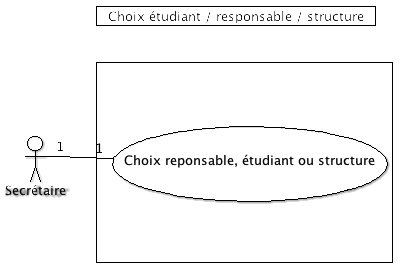
\includegraphics[scale = 0.5]{../UseCase/UseCaseBasNiveau/ChoixEtudiantResponsableStructure.png}
				\caption{Diagrammes représentant les cas d'utilisation à bas niveau}\end{figure}
			
				Une fois l'étape choisie, elle aura accès à la liste des étudiants, des professeurs, ainsi que des UE que regroupe l'étape. Elle pourra alors choisir information qu'elle souhaite parmi une de ces listes.



			\begin{figure}[!h]
\centering	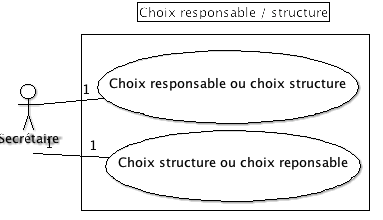
\includegraphics[scale = 0.65]
{../UseCase/UseCaseBasNiveau/ChoixResponsableStructure.png}
				\caption{Diagrammes représentant les cas d'utilisation à bas niveau}\end{figure}
\paragraph{Choix par navigation}

L'utilisateur pourra consulter les données su système à partir d'une interface de navigation en choisissant parmi les différents types de données à sa disposition. Le choix pourra s'effectuer par étudiant, enseignant ou matière. 


\subsubsection{Consultation}

Dans cette section, nous allons aborder les diagrammes de cas d'utilisation liés à la consultation des informations du système.


\begin{figure}[!h]\centering
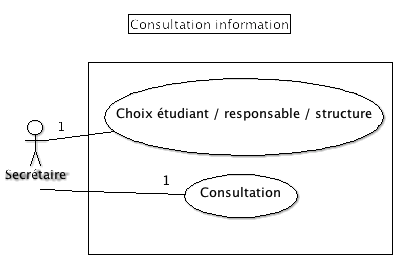
\includegraphics[scale = 0.65]{../UseCase/UseCaseBasNiveau/ConsultationInformation.png}
\caption{Diagrammes représentant les cas d'utilisation à bas niveau}
\end{figure}

\paragraph{Consultation d'informations générales}
Dans la figure précédente, le secrétaire devra choisir par où commencer sa recherche. Les choix qu'il fera lui permettra de restreindre les données cibles. De fait sa recherche s'orientera selon les étudiants possibles, les responsables possibles ou bien les structures d'enseignements possibles.

\begin{figure}[!h]\centering
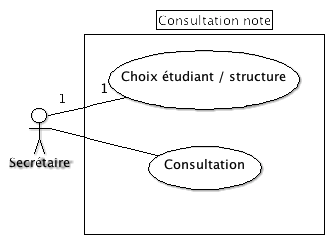
\includegraphics[scale = 0.7]{../UseCase/UseCaseBasNiveau/ConsultationNote.png}
\caption{Diagrammes représentant les cas d'utilisation à bas niveau}
\end{figure}
\paragraph{Consultation de note}~	\paragraph{ } Comme le montre la figure ci-dessus le système permettra la consultation des notes des étudiants via différentes possibilités. Une consultation basique en connaissant le nom de l'étudiant, et une consultation ici d'une navigation à l'intérieur des données.


\begin{figure}[!h]	
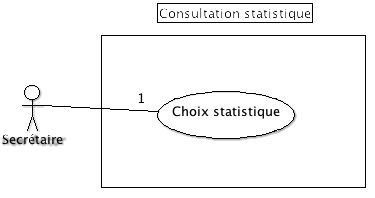
\includegraphics[scale = 0.7]{../UseCase/UseCaseBasNiveau/ConsultationStatistique.png}
\caption{Diagrammes représentant les cas d'utilisation à bas niveau}
\end{figure}

\paragraph{Édition de statistiques}
Comme le montre le diagramme ci-dessus le système permettra l'édition de statistiques prédéfinies et qui ont fait l'objet d'une demande préalable à la conception. Il sera dès lors possible d'obtenir des statistiques basées sur les informations présentes, mais également sur les archives de la base. Des comparaisons seront possibles entre les filières. 
La secrétaire aura alors accès à un ensemble de fonctionnalités telles que les statistiques d'une promotion : résultats, nombre de garçon/fille, études avant Polytech', bourses, nationalité, type d'étude (parcours Polytech ou semestre à l'étranger / Erasmus), ou encore comparer les résultats de différentes promotions. Ces ensembles de fonctions lui permettront bien entendu de pouvoir consulter ou imprimer ces statistiques dans le cadre d'une demande du jury (pour les 
PV par exemple) ou pour des études demandées par Polytech'.


		\subsubsection{L'insertion d'informations}
		
\paragraph{Insertions basiques} Comme le montre la figure ci-dessous, pour insérer de nouvelles données dans le système, il faut au préalable les créer. Une fois ces dernières créées, il sera possible de les insérer dans le système.

\begin{figure}[!h]
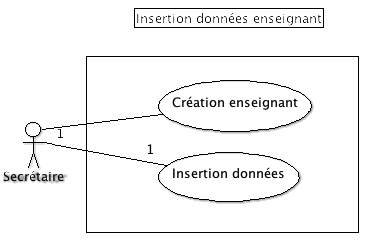
\includegraphics[scale = 0.7]{../UseCase/UseCaseBasNiveau/InsertionDonneesEnseignant.png}
\caption{Diagrammes représentant les cas d'utilisation à bas niveau}
\end{figure}

La création requiert différentes étapes qui seront décrites dans la suite du projet par des diagrammes de séquences.
Nous pouvons cependant en donner une description des à présent. Ici, le secrétaire
pourra se connecter au site, et choisir une étape. Dès lors, il pourra créer un nouvel enseignant.
Une fois créé, un formulaire lui sera présenté qu'elle devra remplir afin de fournir au système les
données sur un enseignant. Enfin, il devra relier cette enseignant à une ECUE pour stipuler qu'il en
est le responsable (cette action peut entrainer la perte de responsabilité d'un autre enseignant, une ECUE n'ayant
qu'un responsable). Dès lors, elle pourra le relier à une UE ou étape s'il doit en être le responsable.


\paragraph{Liaisons des données}~\paragraph{ }La figure ci-dessous nous montre qu'après avoir choisi une structure, il sera possible d'y affecter un enseignant. Ce niveau de détail sera ultérieurement repris par un diagramme de séquences.

\begin{figure}[!h]
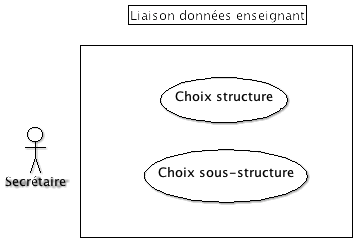
\includegraphics[scale = 0.7]{../UseCase/UseCaseBasNiveau/LiaisonDonneesEnseignant.png}
\caption{Diagrammes représentant les cas d'utilisation à bas niveau}
\end{figure}

Néanmoins, nous pouvons expliquer quelles seront les actions réalisées par le secrétaire.
Après s'être connecté au système, il pourra choisir une étape et lui attribuer un responsable
- soit déjà présent dans la liste, soit en le créant. De même, il pourra choisir une UE ou ECUE de cette étape et
relier la structure à un enseignant déjà existant ou en créant un nouvel enseignant.



	\subsection{Les diagrammes de très bas niveau}

			\begin{figure}[!h]
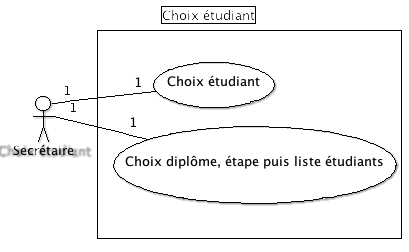
\includegraphics[scale = 0.7]{../UseCase/UseCaseTresBasNiveau/ChoixEtudiant.png}
				\caption{Diagrammes représentant les cas d'utilisation au plus bas niveau}
\end{figure}


Comme le montre la figure ci-dessus, la dernière étape de la consultation se fait soit par le choix de l'étudiant désiré, soit par le choix du diplôme qui débouche sur un choix d'étape puis la liste des étudiants concernés.

\newpage
			
\begin{figure}[!h]\centering
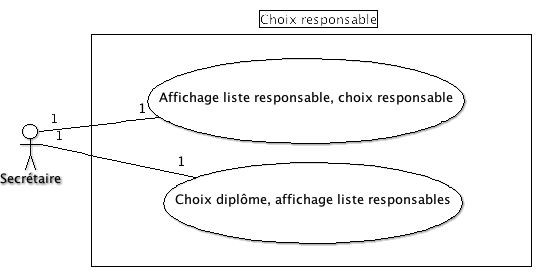
\includegraphics[scale = 0.7]{../UseCase/UseCaseTresBasNiveau/ChoixResponsable.png}
				\caption{Diagrammes représentant les cas d'utilisation au plus bas niveau}
\end{figure}

Comme le montre la figure ci-dessus, la dernière étape de consultation s'effectue avec un choix parmi les responsables ou les diplômes. Ainsi, il n'y a plus qu'à naviguer à l'intérieur des listes pour trouver les données cibles.
Ce diagramme donnera lieu ultérieurement à des diagrammes de séquence pour affiner le niveau de détail. 

			\begin{figure}[!h]	\centering
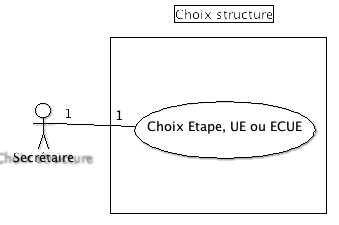
\includegraphics[scale = 0.7]{../UseCase/UseCaseTresBasNiveau/ChoixStructure.png}
				\caption{Diagrammes représentant les cas d'utilisation au plus bas niveau}
\end{figure}

Après avoir choisi de consulter une structure, on peut naviguer dans les étapes rattachées à cette dernière ainsi que les UE ou les ECUE. On finit ainsi la navigation avec les diagrammes de cas d'utilisation.


\section{Les cas d'utilisation pour les enseignants}

Les enseignants n'ont accès qu'à la consultation des ECUE dans lesquelles ils enseignent.
La seule différence est qu'à plus bas niveau, il y a une vérification pour s'assurer qu'il ne puisse consulter que les élèves qui dépendent de lui.
	
	\section{Les diagrammes de collaboration}
	
		Les diagrammes de collaboration permettent de montrer des interactions entre objets, c'est-à-dire des instances de classes et acteurs. Ils permettent de représenter le contexte d'une interaction, car on peut y préciser les états des objets qui interagissent.
		
		Ci-dessous, nous avons représenté divers diagrammes d'activité principalement liés aux notes et à leur gestion. 
		
		\subsection{La consultation des notes}
		
		La consultation des notes, que ce soit pour une promo ou pour un étudiant, sont toutes effectuées de la même façon.
		Le semestre va demander à ses UE de lui donner ses notes. Que ce soit pour une promo ou pour un étudiant particulier, les UE vont alors essayer de calculer leur moyenne : mais pour faire cela, elles nécessitent les notes de chacune des ECUE. Les ECUE à leur tour chercher les notes dans les relations qu’elles ont avec les étudiants. Les étudiants font remonter leurs notes aux ECUE dans lesquelles ils sont inscrits. Les ECUE font remonter le résultat à leur UE respective : cela permet à cette dernière de calculer la moyenne des étudiants qui lui sont rattachés, pondérant chacune des notes avec le coefficient des ECUE la composant. Chacune des UE composant le semestre obtient alors la moyenne des étudiants et font remonter cette information au semestre.
		
		Il est important de noter qu’il existe deux façons de tourner cette fonctionnalité. Nous pouvons travailler à l’échelle d’une promotion, donc calculer à chaque fois les moyennes pour tous les étudiants. Ou bien simplement chercher pour un seul étudiant particulier, et si nous voulons la totalité de la promo, nous itérons cette opération pour chacun des étudiants composant la promotion. Chacune des ces deux méthodes présente des avantages et des inconvénients. Tout dépend de ce que souhaite afficher l’utilisateur : la requête se situera t-elle au niveau d'un seul étudiant, ou bien de la promotion entière ?
				
		Cela revient à dire que la consultation des notes d’un étudiant est une sous fonctionnalité de la consultation globale.
		
		\begin{figure}[!h]
			\centering
				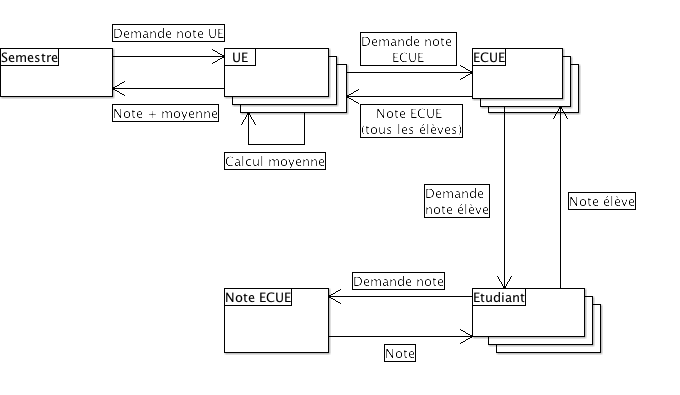
\includegraphics[scale = 0.7]{../Diagrammes_collaboration/Consultation.png}
		\end{figure}
		
		\newpage
		
		\subsection{L'insertion d'une note}
		
		Pour insérer une note, l’enseignant doit transmettre à l’ECUE dont il est responsable une liste d’élèves assortis d’une éventuelle note. L’ECUE prend alors cette liste et pour chaque étudiant va instancier sa note pour l’ECUE en question. 
		
		\begin{figure}[!h]
			\centering
				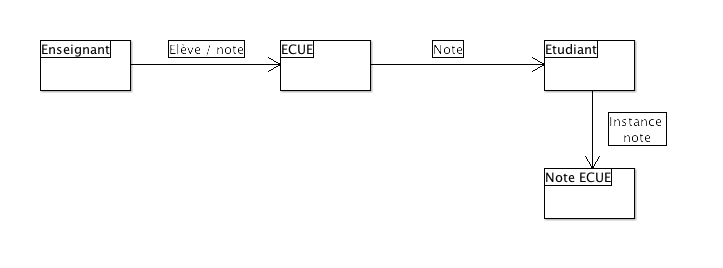
\includegraphics[scale = 0.7]{../Diagrammes_collaboration/Insertion.png}
		\end{figure}
		
		\newpage
		
		\subsection{L'impression du PV}
		
		Pour générer le procès verbal de la promo, il faut travailler au niveau du semestre. En effet, pour le semestre numéro 1, on ne peut générer que la moitié du procès verbal de l’étape. Le fonctionnement actuel permet aux élèves de passer des rattrapages avant la fin du second semestre, et donc d’être capable de générer le PV de l’étape entière. De plus, générer le PV de cette dernière nécessite de le générer pour le second semestre et celui du premier semestre existant depuis quelques mois : une simple concaténation suffit pour obtenir celui de l’étape.
		
	Pour travailler au niveau du semestre, celui-ci demande à ses UE tous les éléments composant la moyenne d'un étudiant. Ainsi, chacune des ECUE demande à chaque étudiant quelle est sa propre note. L’ECUE peut donc renvoyer à son UE la note de chacun des étudiants. L’UE calcule leur moyenne pondérée et renvoie au semestre, pour chaque étudiant, leur moyenne ainsi que chacune des notes des ECUE.	Le semestre n’a plus qu’à assembler les différentes données pour terminer la génération de son propre PV.
		
		\begin{figure}[htbp]
			\centering
				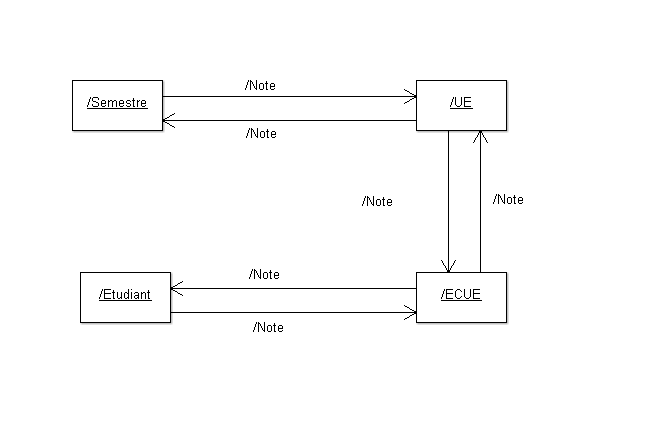
\includegraphics[scale = 0.7]{../Diagrammes_collaboration/Impression_PV.png}
		\end{figure}
		
		\newpage
		
		\subsection{Les rattrapages}
		
		Pour qu’un étudiant puisse effectuer un rattrapage, il doit s’inscrire auprès du responsable de l’ECUE. Ce dernier, à l’issu de l’épreuve, lui attribue une note. Cette modification de note est impactée sur l’UE qui va donc recalculer la moyenne pour tous les étudiants dont les notes ont été modifiées. Une fois les moyennes recalculées, elles sont transmises au semestre en question pour que la nouvelle moyenne des étudiants concernés soit éditée. Les nouvelles moyennes du semestre sont alors impactées sur la moyenne de l’étape pour chaque étudiant.
		
		\begin{figure}[htbp]
			\centering
				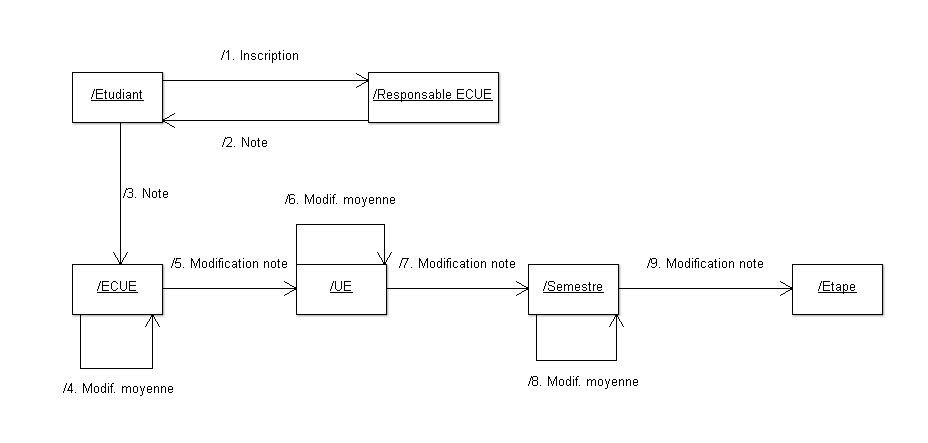
\includegraphics[scale = 0.6]{../Diagrammes_collaboration/Rattrapages.png}
		\end{figure}
		
		\newpage
		
		
		
		\subsection{L'admission en année supérieure}
		
		Pour savoir si un étudiant est admis en année supérieure, il doit avoir validé chacune de ses UE. c'est-à-dire obtenir au moins 10 à chacune et avoir une moyenne au semestre de 12 minimum. Pour vérifier tout cela, il est demandé à l’UE d’envoyer au semestre pour chacun des étudiants de ce dernier, la note à l’UE, ainsi que les éventuels points jurys. Le semestre récupère ces informations et va les transmettre la moyenne du semestre, ainsi que les éventuels points jurys à l’étape qui pourra vérifier que les étudiants sont admis.
		
		\begin{figure}[!h]
			\centering
				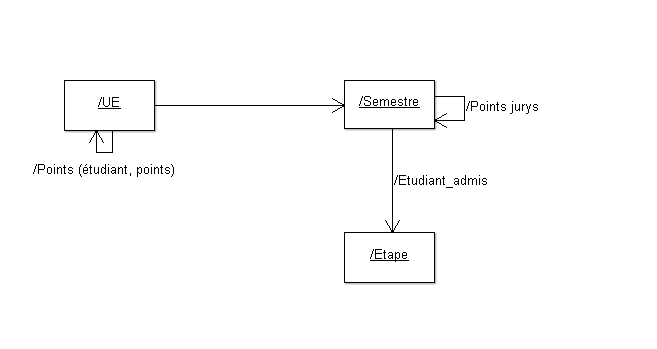
\includegraphics[scale = 0.7]{../Diagrammes_collaboration/Admission_en_sup.png}
		\end{figure}
		
		\newpage
	
	\section{Les diagrammes de séquence}
	
		\subsection{Choix de l'action à réaliser}
		
		Les différents cas d’utilisations étant nombreux, il était nécessaire de réaliser un premier diagramme de séquence visant à expliquer les premiers choix qui s’offraient à l’utilisateur. En effet, l’insertion de note peut s’effectuer de différentes manières : par élève, par promotion (avec une feuille Excel) ou par ECUE. C'est-à-dire qu'il est possible (dans le cas d’un rattrapage par exemple) d'insérer une note pour un élève donné. Nous pourrons alors choisir dans quelle ECUE rentrer cette note, ou choisir l’ECUE dans laquelle nous voulons insérer la note, puis l’élève correspondant.
		Nous retrouve donc ici ces différents choix, permettant d’offrir toutes les possibilités de fonctionnalité à l’utilisateur.
		
		\begin{figure}[htbp]
			\centering
				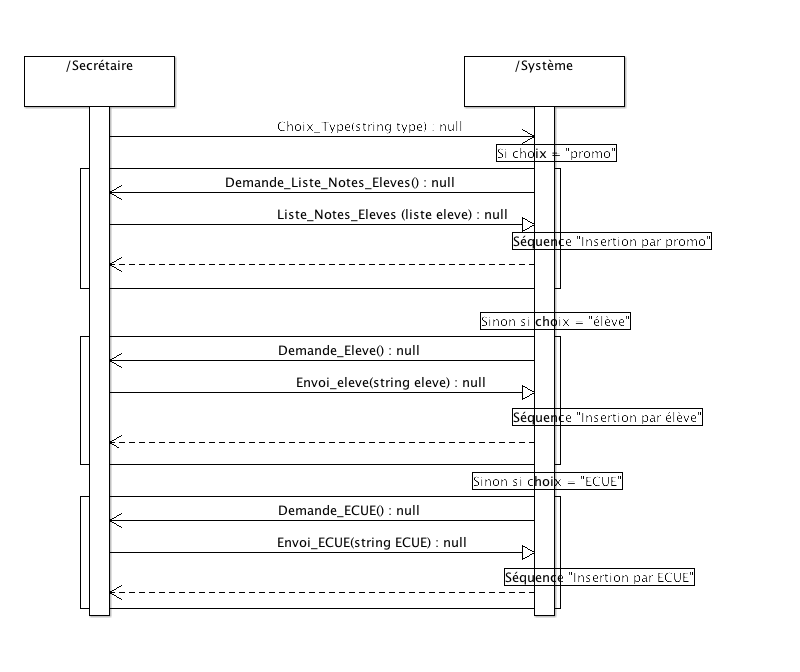
\includegraphics[scale = 0.6]{../Diagrammes_sequence/Diagramme_sequence_choix_action}
		\end{figure}
		
		\newpage
		
		\subsection{Insertion par promotion}
		
		Ce diagramme vient compléter celui précédemment expliqué. Il s’agit d’insérer l’ensemble des notes de la promotion pour une ECUE donnée. 
		
		L’utilisateur insère donc sa liste de notes (par feuille Excel par exemple). 
		Le système lui demande pour quelle ECUE est cette liste de note : une fois l’ECUE trouvée, le système lui envoie la liste des notes. 
		L’ECUE pourra alors remplir sa liste de notes en recherchant chaque étudiant et en créant avec eux un objet "note" qui correspond à la note de l’étudiant pour l’ECUE. L’opération se répète ainsi pour tous les étudiants, en relevant d’éventuelles erreurs qui pourraient survenir dans le cas où la liste donnée par la secrétaire ne correspond pas réellement à la liste des élèves de l’ECUE.
		
		\begin{figure}[htbp]
				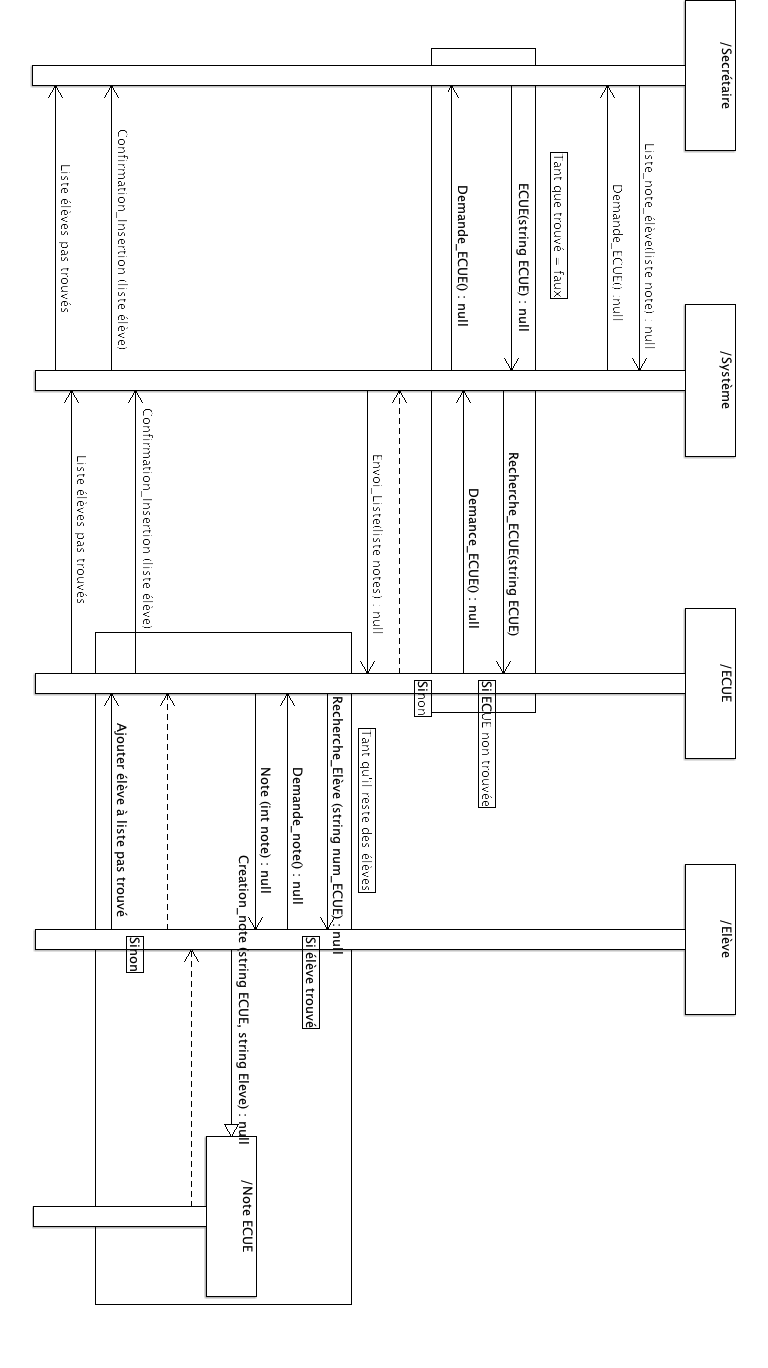
\includegraphics[scale = 0.5]{../Diagrammes_sequence/Diagramme_sequence_insertion_promo.png}
		\end{figure}
		
		\newpage
				\subsection{Insertion par ECUE}
		
		Ce diagramme correspond à l’insertion d’une note pour un élève et une ECUE donnée. Il met en avant l’insertion d’une note pour une ECUE en passant par un élève, et est complété par le diagramme suivant ("Insertion par ECUE) qui réalise le même cheminement mais en passant tous d’abord par une ECUE avant d’atteindre l’élève.
		
		Partons donc du principe que l’utilisateur choisit d’abord un élève. Le système va alors chercher l’étudiant : si ce dernier n’existe pas en mémoire, il va redemander un élève correct. Une fois cet élève trouvé, il va demander l’ECUE sur laquelle portera sa note, puis la chercher. Une fois cette dernière trouvée, il pourra  demander la note. Cette dernière sera envoyée à l’élève qui la transmet à l’ECUE, qui va elle-même créer une note ECUE pour l’élève qui lui aura transmis sa note.
		
		
		\begin{figure}[htbp]
				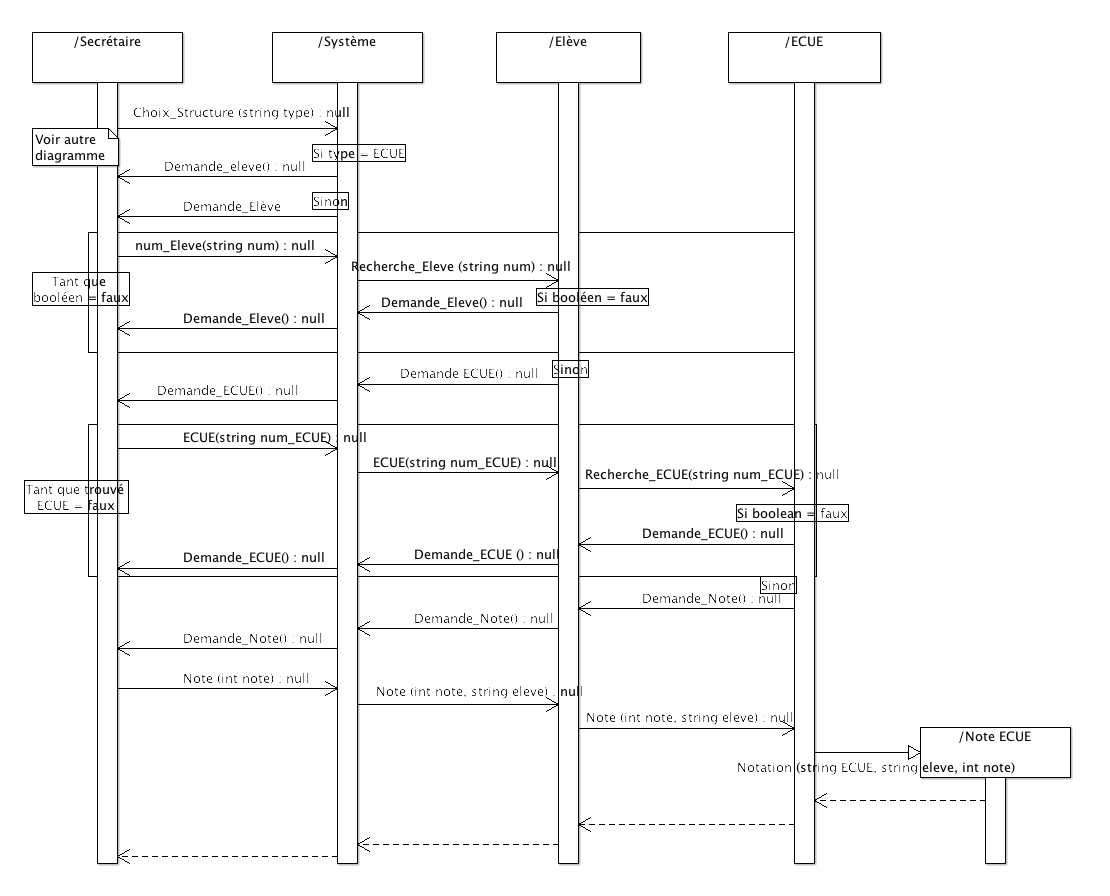
\includegraphics[scale = 0.53]{../Diagrammes_sequence/Diagramme_sequence_insertion_eleve.png}
		\end{figure}
		
		\newpage
		
		\subsection{Insertion par élève}
		
		Ce diagramme correspondant au même processus que le précédent. La seule différence notable ici c’est que l’utilisateur choisit tout d’abord l’ECUE pour laquelle il veut noter un élève. Une fois trouvée, il choisit l’élève en question. Dès lors, il demande la note qu’il passera à l’ECUE, qui elle-même la transmettra à l’élève afin qu’il crée une note correspondant à sa note dans l’ECUE appelante. 
		
		\begin{figure}[htbp]
				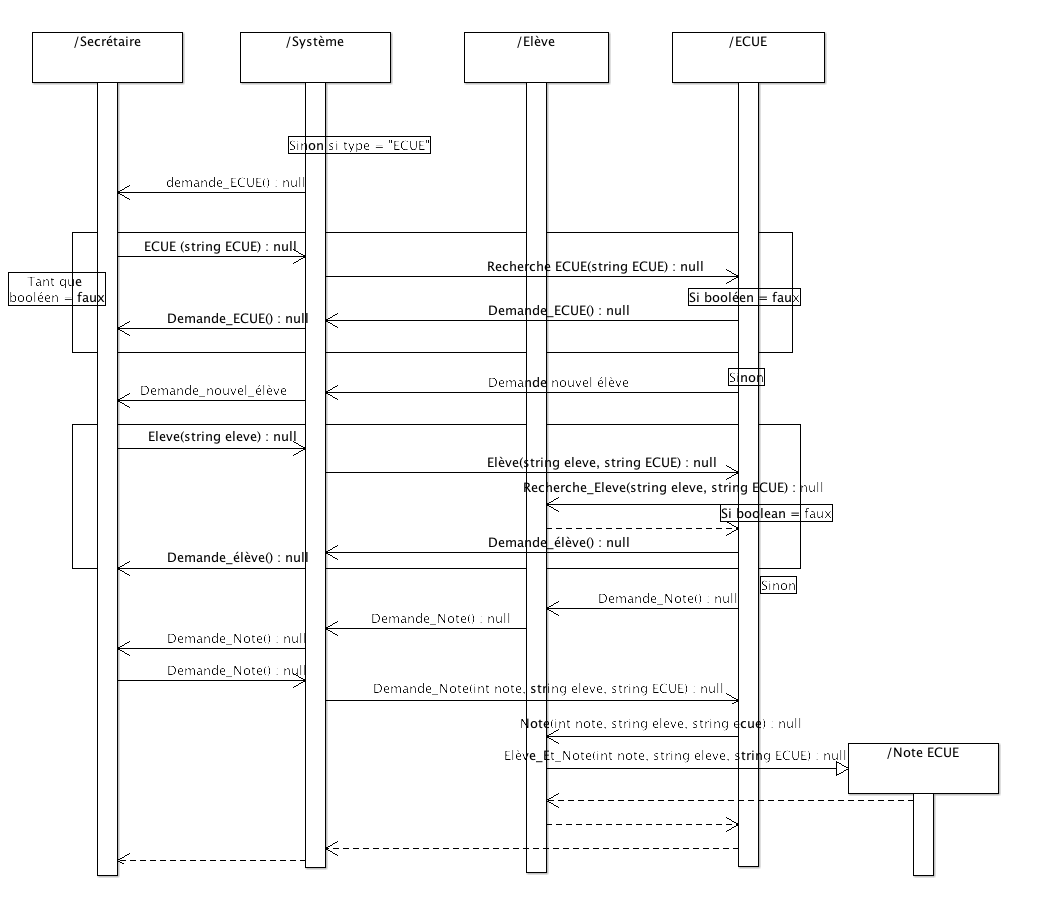
\includegraphics[scale = 0.53]{../Diagrammes_sequence/Diagramme_sequence_insertion_ECUE.png}
		\end{figure}
		
		\newpage
		
		\subsection{Les points jurys}
		
		Ce diagramme représente un exemple d’insertion des points jury pour une UE et pour un élève. Bien sur, ce n’est pas le seul cas possible, mais il permet de bien comprendre le cheminement, et, les autres cas étant sensiblement les mêmes, nous avons jugé qu’il était suffisant d’en exposer un seul.
		La secrétaire décide donc ici d’ajouter des points jury à un élève pour une UE. Le système va alors rechercher l’élève pour lui transmettre l’information. Ce dernier signalera dès lors à l’UE pour laquelle ses points jury on été ajouté la modification. L’UE instanciera alors les points jury de l’élève. Ici, la communication se fait en demandant d’effectuer une action. Seule l’UE déclenche réellement une action sur les points jury en leurs demandant de se mettre à jour. Les retours ne sont donc pas demandé par les classes appelante, mais effectué à l’initiative des classes appelé si besoin est (pour stipuler que le changement à bien eu lieu et en donner le résultat par exemple).
		Il est à présent important de donner la liste exhaustive des cas similaire pouvant ce présenter. Un secrétaire peut vouloir, pour un élève, ajouter ou modifier les points jury, et ce pour une UE ou un semestre. Dans chacun de ces cas, elle peut décider de choisir tous d’abord l’UE ou le semestre, puis l’élève, ou l’inverse.
	
		
		\begin{figure}[htbp]
				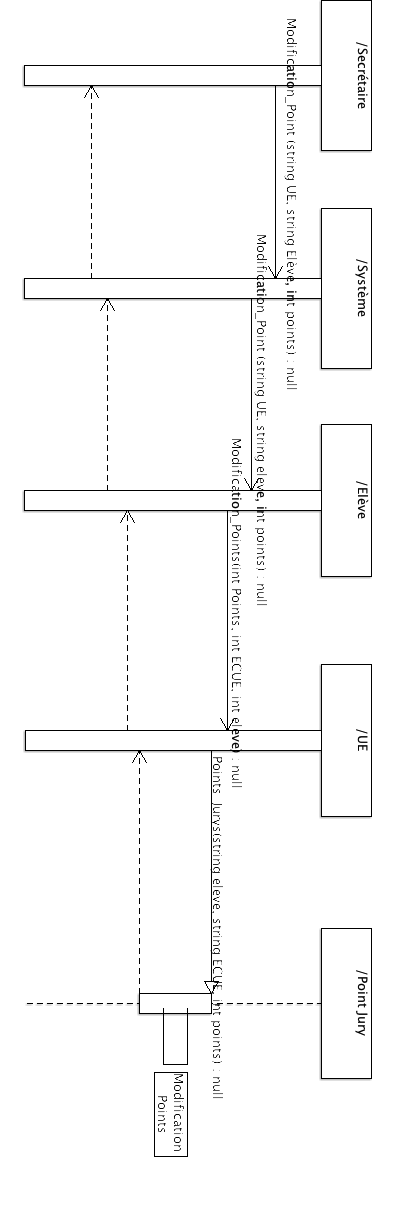
\includegraphics[scale = 0.55]{../Diagrammes_sequence/Diagramme_sequence_points_jurys}
		\end{figure}
		
		\newpage
		
		\subsection{Demande de PV}
		
		Le dernier diagramme est la demande du PV. L’utilisateur peut demander le PV pour une promotion et un semestre. Dès lors, le système recherche le semestre en question, et lui demande l’ensemble de ses notes. Le système va dans un premier temps parcourir l’ensemble de ses UE en leur demandant à leur tour leurs notes. Ces dernières vont parcourir toutes leurs ECUE afin de récupérer les notes. Une fois les notes récupérées, l’UE va calculer la moyenne de chaque étudiant (à l’aide des notes des ECUE récupérées et des coefficients ECUE) puis renvoyer le tout (notes ECUE + moyenne UE) au semestre. Une fois toutes ces données récupérées, le semestre va à son tour calculer la moyenne de chaque étudiant et renvoyer le tout au système qui disposera alors de toutes les informations pour réaliser le PV.
		
		\begin{figure}[htbp]
				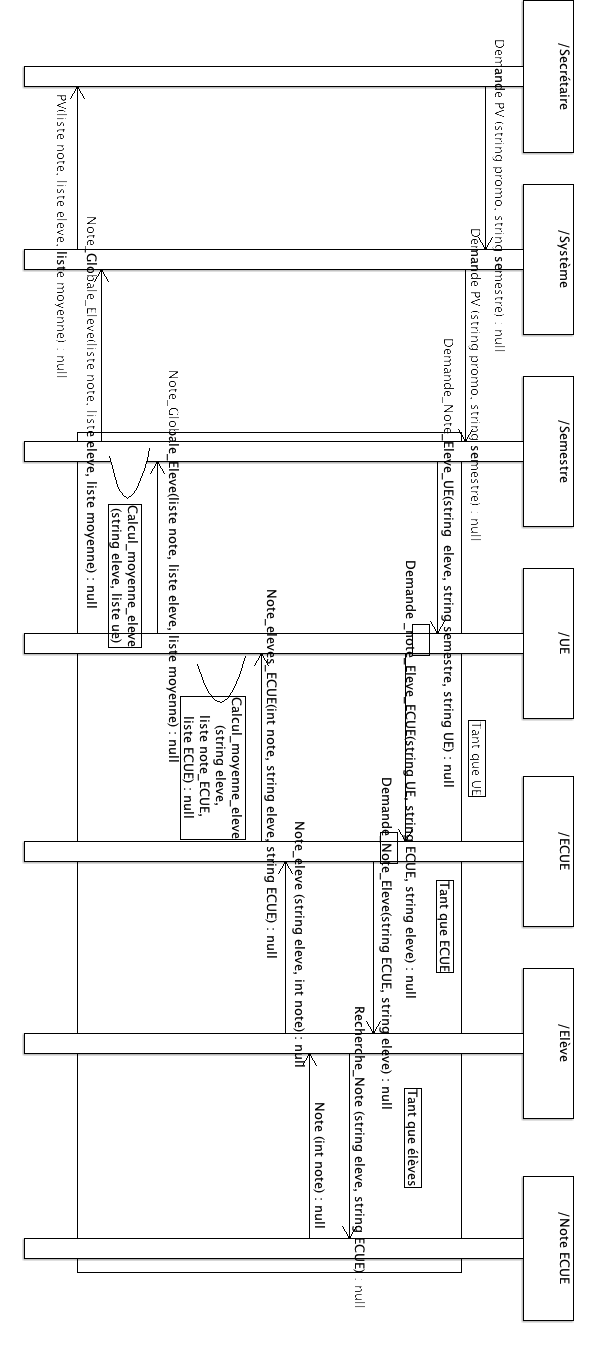
\includegraphics[scale = 0.4]{../Diagrammes_sequence/Diagramme_sequence_demande_PV.png}
		\end{figure}
		
		\newpage
	
	\section{Le diagramme d'activité}
	
	Notre diagramme a été divisé en deux parties pour des raisons pratiques, mais les deux se recoupent. Ce diagramme représente le processus de gestion des notes, et points jury d’un étudiant et validation des acquis tout au long d’une année. Le déroulement général (simplifié) du processus suit les étapes suivantes :
	\begin{itemize}
		\item{Extraction et initialisation des données concernant l’étudiant et les structures pédagogiques}
		\item{Notations pour le premier semestre}
		\item{Jury et rattrapages après premier semestre}
		\item{Notations pour le second semestre}
		\item{Jury et rattrapages après le second semestre}
		Dans le cas de la formation FQSC, un seul semestre est effectué et il y a donc un seul jury et une session de rattrapages.
	\end{itemize}
	
		\subsection{Notation d'un semestre}
		
		Le système de notations du premier et du deuxième semestre sont en tout point similaires. 

			\subsubsection*{Le cas classique}
			
		La note d’un semestre est, de façon générale, calculée à partir de la note de l’étudiant dans chacune des Unités d’Enseignement (UE) du semestre.
		Pour cela, il faudra attribuer les notes des UE une par une, en choisissant l’UE parmi la liste proposée. En cas d’erreur, l’UE pourra être de nouveau sélectionnée pour en modifier la note.

			\subsubsection*{Le cas des stages de redoublement}
			
		Il existe cependant une exception : si l’étudiant est redoublant et qu’il a les acquis pour le semestre en cours (il redouble à cause de l’autre semestre), les cours et examens du semestre peuvent lui être dispensés au profit d’un stage. Dans ce cas, il n’a donc pas de notes pour les UE et les ECUE du semestre, et sa note du semestre est constituée uniquement de sa note de stage.
		
		\subsection{Notation d'une UE}
		
		\subsubsection*{Le cas classique}
		
		De manière générale, la note d’une UE est issue d’un calcul entre les notes des ECUE la composant. On doit donc rentrer une par une les notes des ECUE après les avoir sélectionnées. Les ECUE peuvent être resélectionnées et leur note modifiée en cas d’erreur.

		\subsubsection*{Un cas variant}
	
		Dans certains cas exceptionnels, les notes d’ECUE ne sont pas entrées : on rentre directement la note de l’UE.
		
		\newpage
		
		\begin{figure}[htbp]
				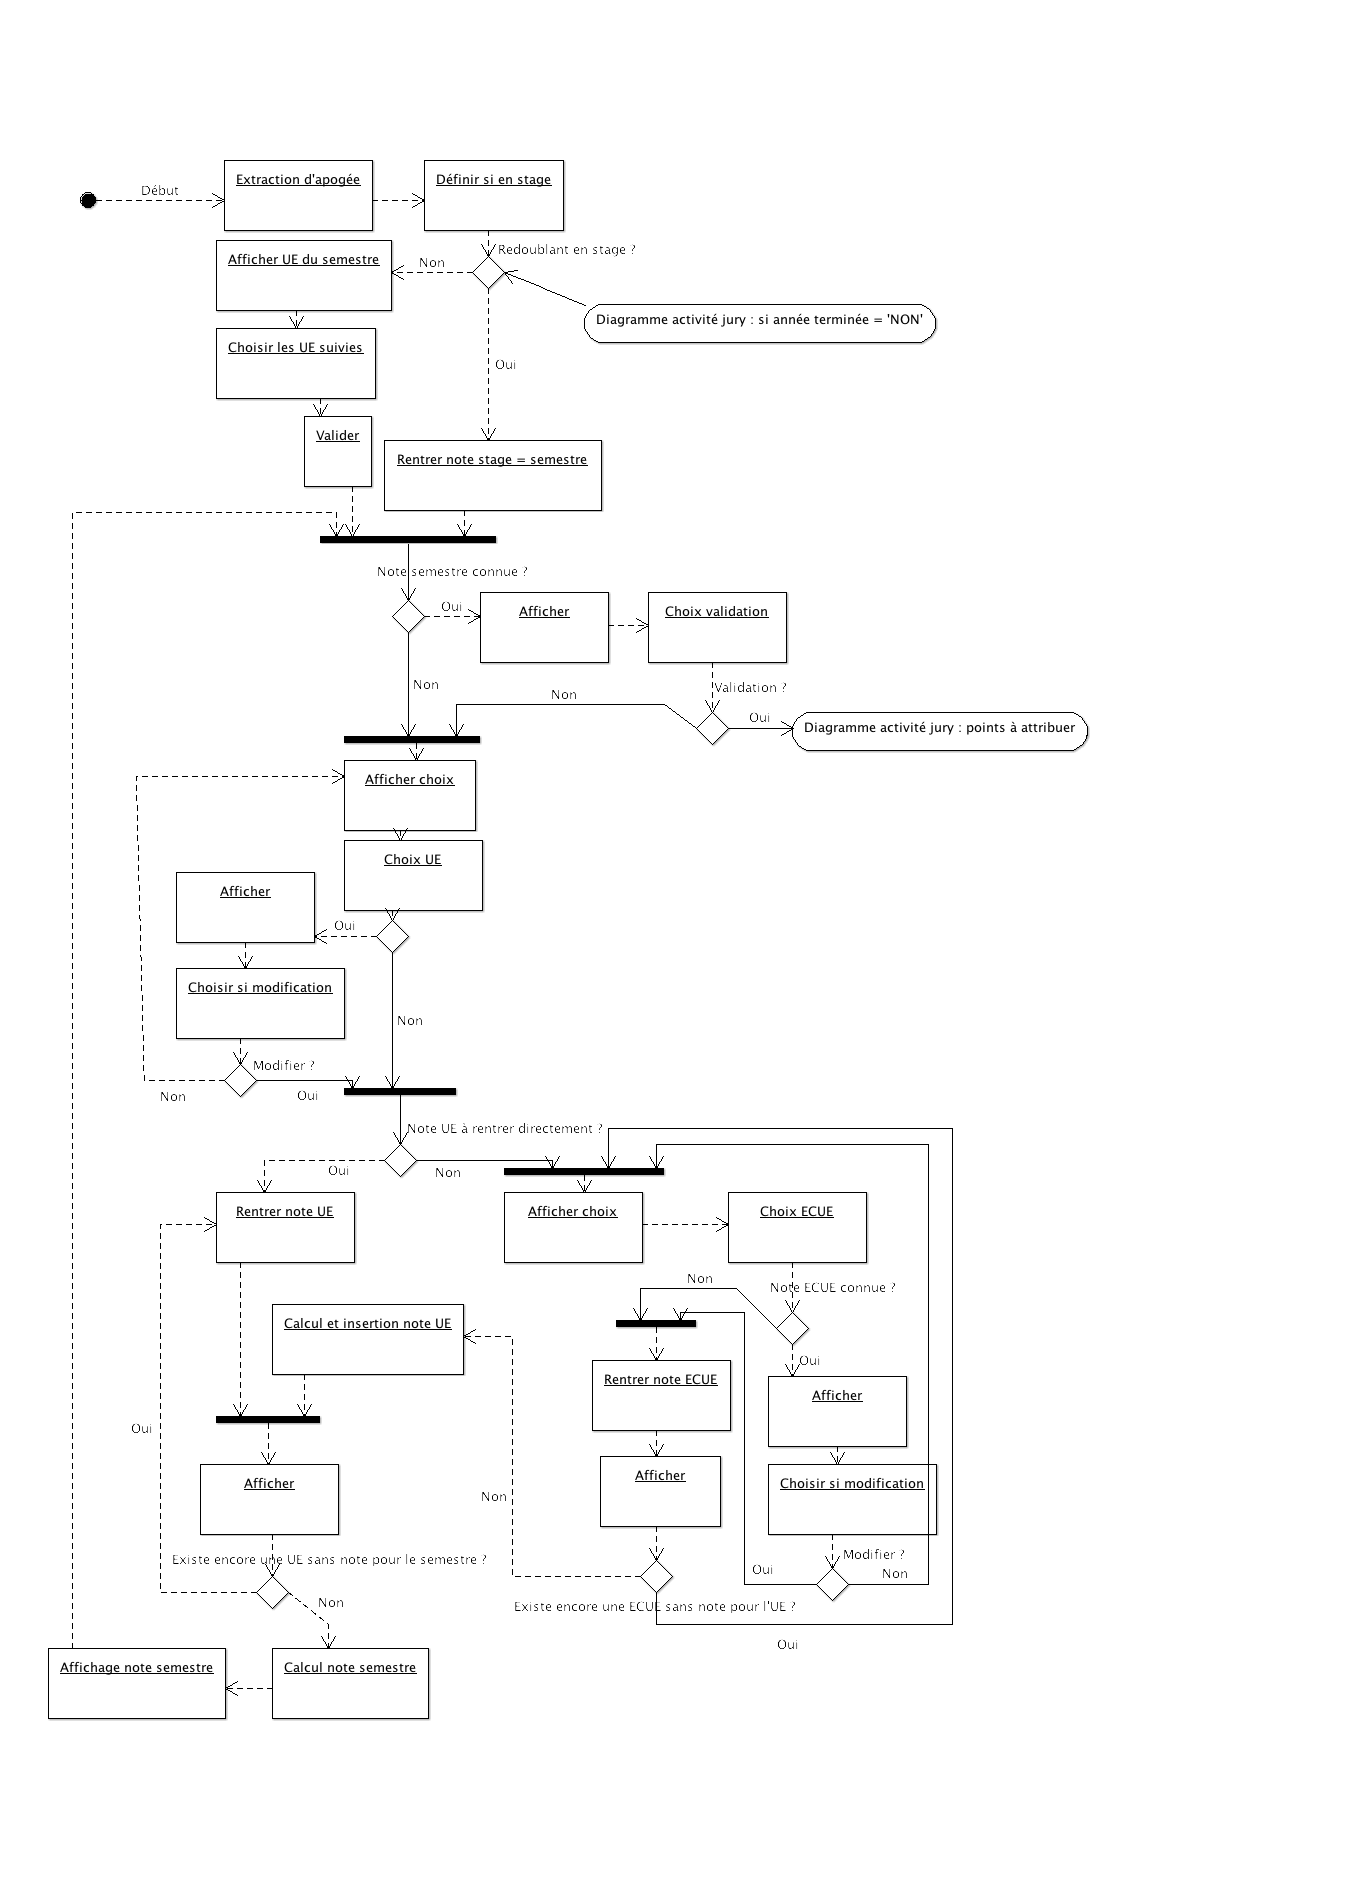
\includegraphics[scale = 0.4]{../Diagramme_activite/Diagramme_notation.png}
		\end{figure}
		
		
		\subsection{Le jury}
	
		Il existe trois cas que nous allons détailler :
		\begin{itemize}
			\item{Semestre acquis par validation}
			\item{Semestre non acquis par validation, mais acquis par décision du jury}
			\item{Semestre non-acquis.}
		\end{itemize}

			\subsubsection*{Semestre acquis par validation}

		C’est le cas le plus courant : l’élève a plus de 12 de moyenne au semestre et a plus de 10 dans chacune des UE. On lui attribue la mention “Acquis” pour chacune des UE.

			\subsubsection*{Semestre acquis par décision du jury}

		Cela signifie que l’élève n’a pas réussi son semestre (12 de moyenne et 10 dans chaque UE), mais qu’on lui accorde sa validation tout de même. Cette situation est possible dans trois cas :
		\begin{itemize}
			\item{soit le jury fait preuve de clémence et lui accorde des points supplémentaires sans lui demander de passer des repêchages (à des UE en modifiant les notes ou à des semestres)}
			\item{soit l’élève réussit à remonter ses notes grâce à des repêchages}
			\item{soit l’élève passe des repêchages, n’a pas de notes suffisantes, mais le jury lui accordent   quand même des points supplémentaires de façon à ce que son semestre soit validé}
		\end{itemize}


		Nous allons présenter les différentes étapes qui mènent à la validation d’un semestre par décision du jury.
		On attribue tout d’abord à l’étudiant la mention “Acquise” pour chacune des UE où la note est au-dessus de 10.

		Si l’élève possède au moins une UE dont la note est inférieure à 10, le jury peut décider de modifier des notes d’UE de façon à ce qu’il ait 10 dans ces UE. Dans ce cas, la mention “Acquis par Décision du Jury”(ACDJ) est attribuée à l’élève pour les UE en question. Le jury peut ensuite décider d’attribuer des points au semestre si nécessaire pour faire en sorte que la note de 12 soit atteinte (il n’est pas possible d’ajouter des points semestre si cela ne fait pas passer la note à 12).

		Après ces décisions du jury, on vérifie que les UE soient toutes “Acquises” ou “ACDJ”, et que la note de semestre soit supérieure à 12. Si ce n’est pas le cas, des rattrapages sont nécessaires. Après ses rattrapages, les notes de rattrapage sont rentrées (en parallèle à la note initiale), ce qui modifie les notes d’ECUE, d’UE, de semestre. Si ces modifications font passer certaines notes en dessous de 10, la mention “Acquise” ou “ACDJ” doit être retirée. Au contraire, on ajoute la mention “ACDJ” aux UE qui n’avaient pas de mention (éventuellement, le jury aura pu modifier la note d’UE avant).

		Des points jury peuvent être attribués au semestre de la même façon qu’avant les rattrapages.


		Il est important de noter que l’important à Polytech n’est pas d’avoir 12 à chaque semestre pour passer à l’année suivante, il faut juste avoir 12 sur l’année (la moyenne des deux moyennes de semestre). Ainsi, un étudiant peut avoir 11 au premier (après rattrapages et actions ou non du jury) et continuer son année, puis avoir 13 au second et passer à l’année supérieure. Il faut cependant faire attention et accorder des rattrapages de second semestre à un élève qui n’aurait que 11 au premier et 12,5 au second : ce n’est pas parce que 12,5 est supérieur à 12 qu’il faut priver l’étudiant de rattrapages pour faire passer sa moyenne annuelle à 12.

		\subsubsection*{Semestre non-acquis}

		L’étudiant, malgré la possibilité qu’a eu le jury de lui rajouter des points et malgré les deuxièmes sessions d’examen qui lui ont été accordées (voir “Semestre acquis par décision du jury”), n’est pas parvenu à faire passer la note d’un de ses semestres au dessus de 12, même par compensation avec l’autre semestre, le semestre est considéré comme non-acquis et l’étudiant redoublera ou sera exclu.

		Cette situation peut aussi arriver si le semestre contient une UE pour laquelle l’étudiant n’a pas eu la note minimale de 10 (deuxièmes sessions, et points du jury n’auront pas suffi).	

		
		\begin{figure}[htbp]
				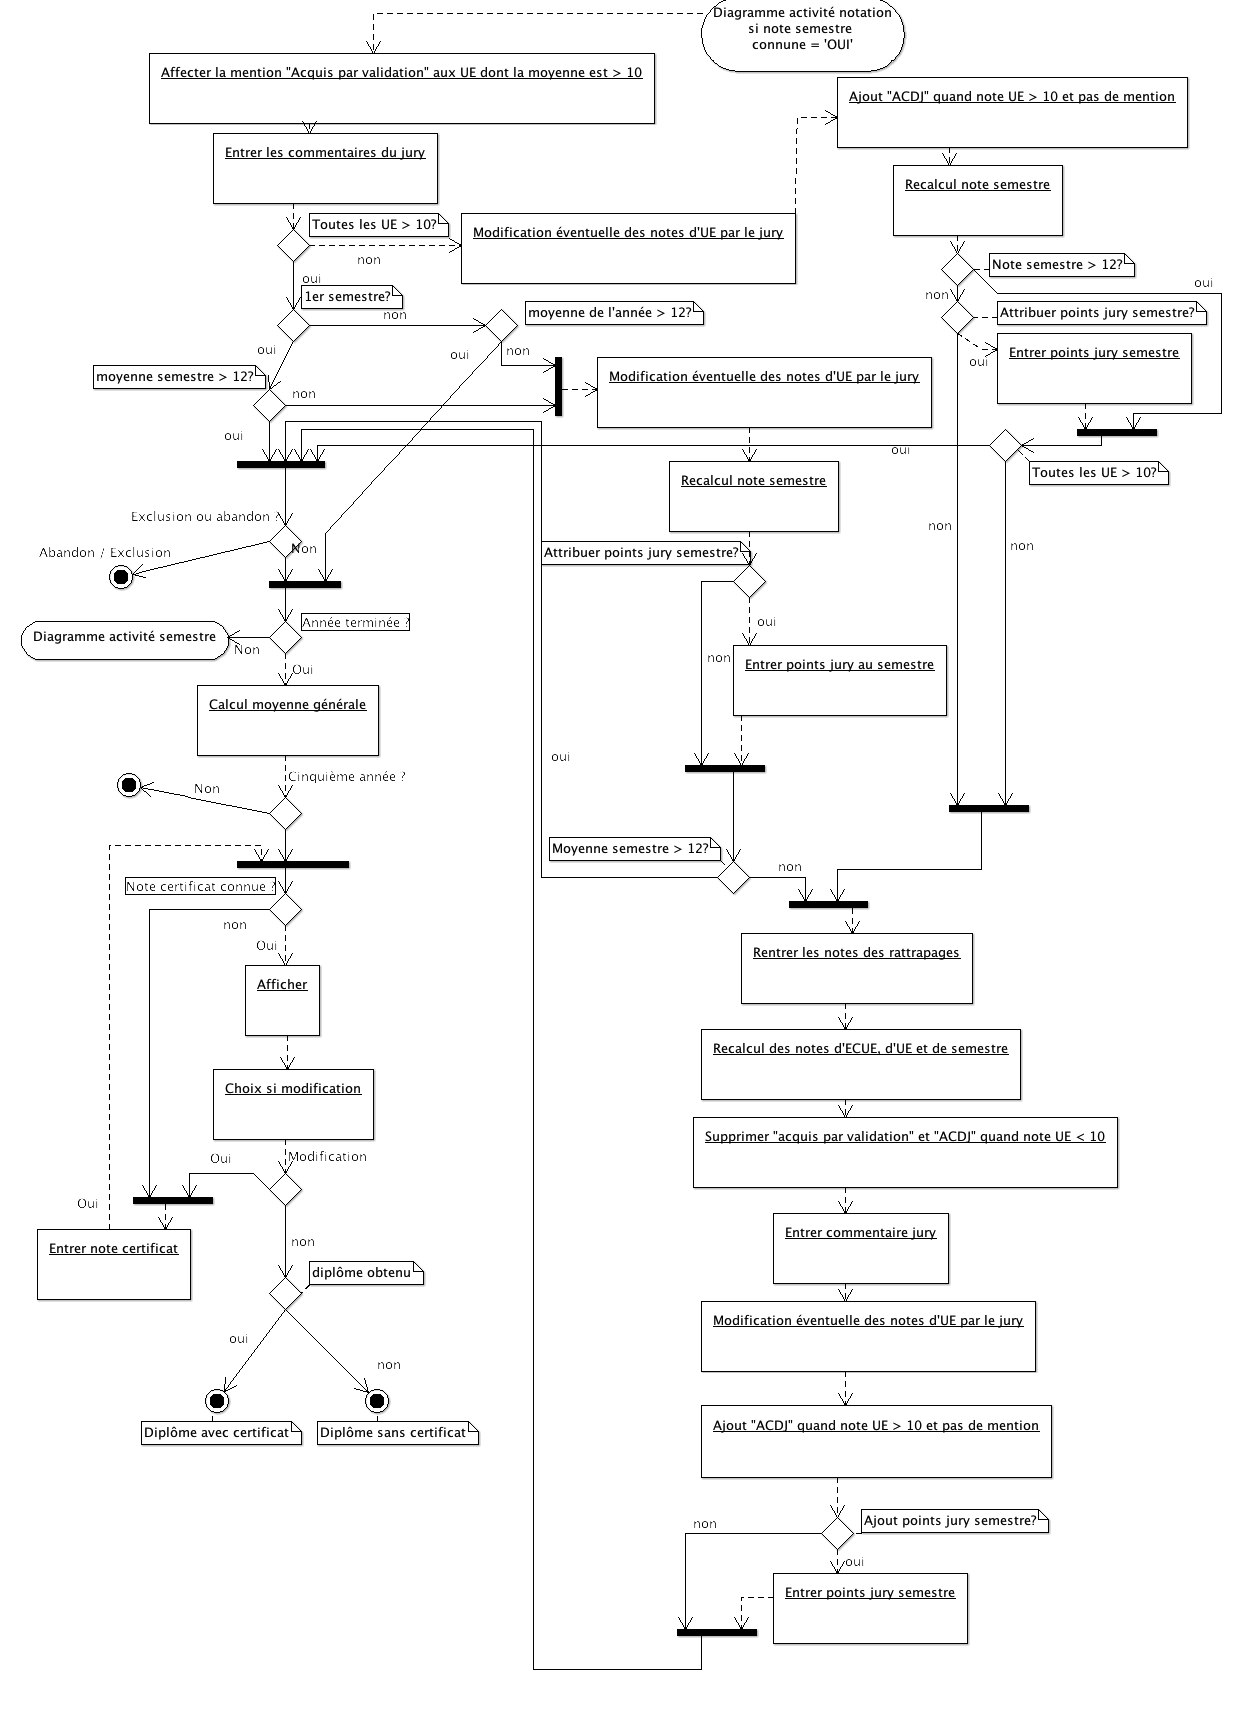
\includegraphics[scale = 0.4]{../Diagramme_activite/Diagramme_jury.png}
		\end{figure}
		
		\newpage
	
	\section{Le diagramme de machines d'état}
	
	Le diagramme de machines d'état correspond, dans une certaine mesure, à une sorte d'organigramme dédié à ce qui était autrefois appelé la programmation structurée. Ici, notre diagramme correspond au parcours d'un étudiant, pour chaque année et ce jusqu'à la fin de son cursus.
	Le point de départ consiste en l'extraction de l'étudiant du logiciel Apogee. Etant donné qu'il est déjà inscrit au moment où il va commencer son son année, cette étape est gérée par ce logiciel.

	A partir du moment où l'étudiant est extrait, il va être noté pour chacune de ses ECUE. Nous allons donc créer des instances des classes concernées, et ce jusqu'à ce que toutes les notes des ECUE soient connues. Nous ne passons donc pas à l'instanciation d'une note d'UE tant que la totalité des notes d'ECUE ne sont pas données. Dans le même laps de temps, il est possible que l'étudiant passe son certificat. A la suite de quoi nous allons instancier la classe concernant cet examen.

	Lorsque cette étape est terminée, toutes les notes d'UE sont calculées. Ceci étant fait, nous pouvons instancier la note du semestre.
	C'est le jury qui décide de la suite du cursus : si l'étudiant a obtenu la moyenne générale satisfaisante, ainsi que pour chacune de ses UE, l'étudiant va pouvoir directement bénéficier de l'état d'admission au semestre.
	Mais s'il manque des points à l'élève, celui-ci pourra bénéficier de certains points donnés par les jurys, ce qui lui permettra d'obtenir l'admission au semestre.

	Si l'élève ne rentre dans aucun de ces deux cas, il devra passer par les rattrapages. Au point de vue du diagramme, ceci va consister à instancier l'ensemble des notes qu'il a obtenu lors de cette session, c'est-à-dire de modifier les notes qu'il a obtenu dans les ECUE. Une fois que l'ensemble des rattrapages sont effectués, l'étudiant sera admis pour le semestre 2 quels que soient les résultats obtenus. Ce qui permet à l'étudiant de pouvoir se rattraper s'il manque uniquement des points concernant la moyenne générale, et de compenser lors du second semestre.

	Le deuxième semestre n'ayant aucune différence particulière avec le premier, nous avons fait le choix de reprendre un système identique. Ceci permet à notre schéma de rester le plus générique possible. Nous effectuons donc l'instanciation d'ECUE et du certificat (si nécessaire), puis l'instanciation d'UE pour arriver au semestre. Les potentiels rattrapages donnent toutefois lieu à l'état "Admis semestre 2". Ce qui veut dire que l'étudiant a terminé son semestre. C'est lors de l'instanciation de la moyenne générale de l'étudiant - la note de l'étape - que l'état final va déterminer la fin d'année de l'étudiant.
	Si celui-ci n'a pas été admis pour l'année, il sera alors dans l'état "Redoublement" et devra refaire l'année.
	
	Si l'élève a obtenu son année, en revanche, divers choix s'offrent à lui. Soit l'élève est dans l'un des cursus entre la première et la quatrième année, auquel cas il pourra normalement passer à l'année suivante.
	Si l'étudiant est en cinquième année, en revanche, deux états finaux sont possibles. Soit il a passé le certificat et il peut obtenir son diplôme normalement, soit il dispose du statut "Diplôme obtenu sans certificat". Ce sera alors à lui de passer le diplôme, plus tard, afin de valider complètement le diplôme. Toutefois, ce n'est pas à prendre en compte dans le cursus d'une année à passer à Polytech', d'où la non prise en compte dans le diagramme ci-dessus.

	Nous noterons aussi qu'il est possible qu'à chaque étape, l'étudiant peut être exclu du cursus qu'il suit. Cela implique évidemment une faute grave de sa part, mais étant donné que cela peut arriver à tout moment de l'année, il apparaît comme état final pour chaque état du cursus suivi.
	En revanche, l'état d'abandon d'un étudiant n'est signalé qu'au jury de chaque semestre. Il est donc inutile de le mettre en évidence comme il l'est effectué pour l'exclusion.
	
	\begin{figure}[htbp]
			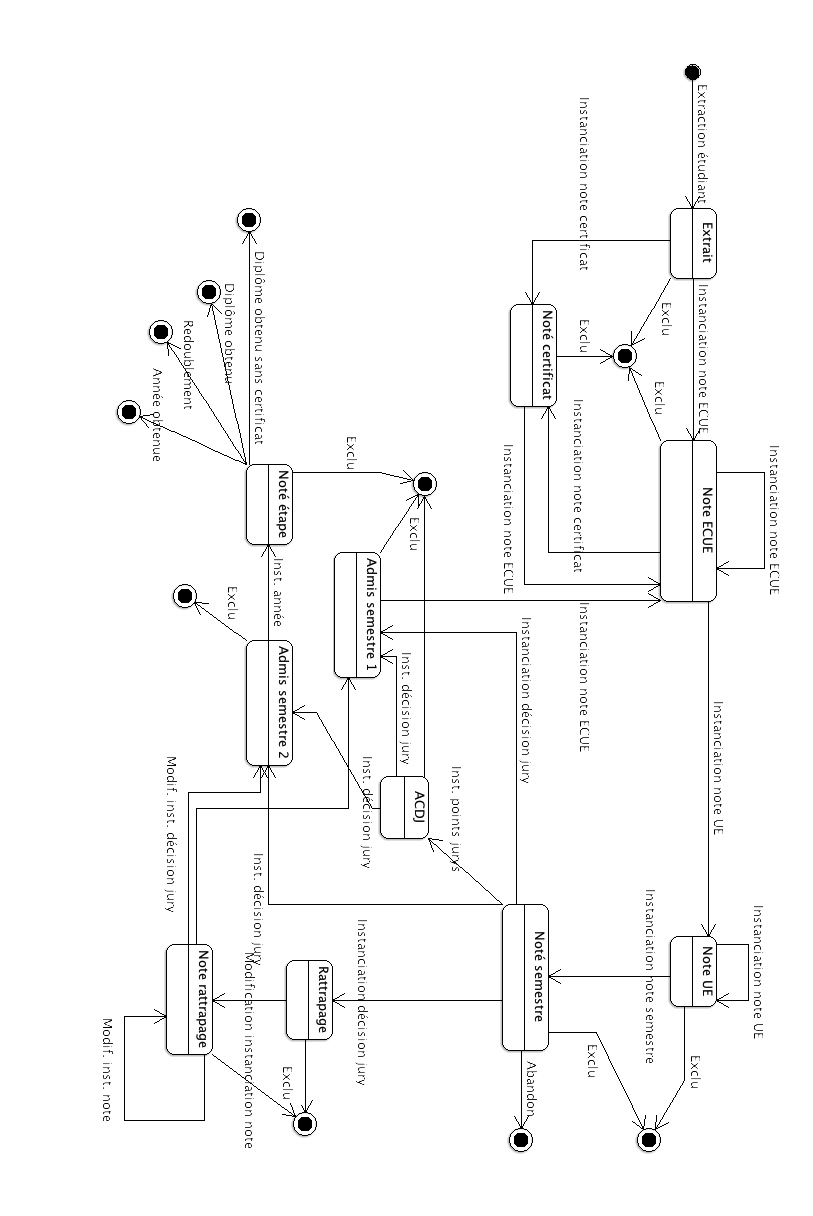
\includegraphics[scale = 0.6]{../Diagramme_machine_etat/Machine_etat.png}
	\end{figure}
	
	\newpage
	
	\section{Conclusion du rapport d'activité}
	
	Une fois le diagramme de classes établi, ces différents diagrammes nous ont paru plus évidents à réaliser. Les diagrammes de séquence et de collaboration nous permettent, comme pour le diagramme de machine d'état, de mieux visualiser les différents liés établis entre les classes, en les instanciant pour passer de l'une à l'autre. Les diagrammes de collaboration. Le diagramme d'activité, quand à lui, se positionne plutôt du côté utilisateur, afin de relever l'activité réalisée par l'utilisateur, comme nom nom l'indique. 
	
	Avec l'ensemble de ces diagrammes, nous pouvons donc entamer la partie de développement de manière confiante, car nous disposons maintenant de bonnes bases. De plus, ceci nous a permis de mieux comprendre l'utilité des différents diagrammes, et nous saurons maintenant les utiliser à notre gré pour développer le logiciel.
	
	\section{Bilan du projet transversal}
	
	Il est très intéressant de pouvoir se rendre compte de l'évolution de la conception d'un tel projet. Mais il est d'autant plus intéressant de voir comment passer de la conception au développement, afin de concevoir le logiciel dans son intégralité. Nous avons pu nous approcher de la phase de développement, en réfléchissant à la manière d'implémenter les fonctionnalités. Toutefois, nous devons avouer que cela ne nous a pas toujours semblé facile, et que nous n'étions pas trop de quatre pour réfléchir et débattre pour chacun des diagrammes à réaliser. Mais chacun de nous a saisi l'utilité de ces derniers pour la phase de développement. Bien que nous n'ayons pas été amené à effectuer des phases de test ou de dialogues avec le client, cela nous donne une bonne vision des tâches que nous serons amenés à effectuer plus tard. 
	
	Même si nous jugeons que certaines phases du projet auraient pu être menées avec plus d'efficacité, nous sommes toutefois satisfaits du travail que nous avons réalisé. Nous espérons donc que vous êtes satisfaits du travail que nous avons réalisé, et devons maintenant nous atteler au développement du logiciel dans les plus brefs délais.
		
\end{document}
					
